\documentclass{standalone}
\usepackage{tikz}
\usetikzlibrary{patterns, positioning}

\begin{document}
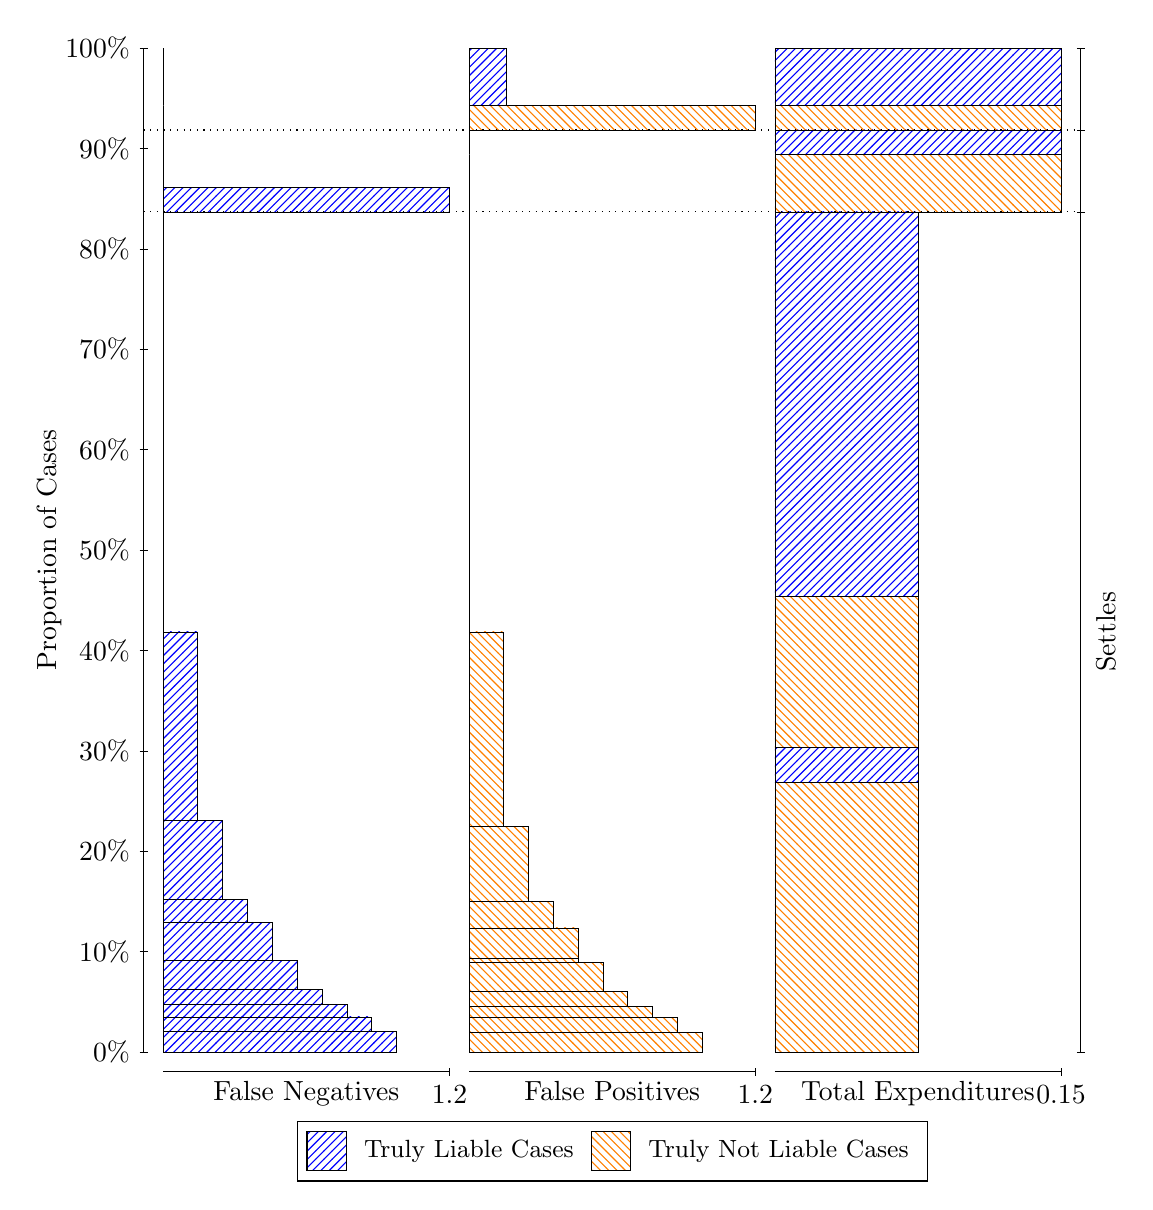
\begin{tikzpicture}
\draw[black, very thin] (1.5,1.75) -- (1.5,14.5);
\node[rotate=90, anchor=center] at (0.3, 8.125) {Proportion of Cases};
\draw[black, very thin] (1.45,1.75) -- (1.55,1.75);
\node[anchor=east] at (1.45, 1.75) {0\%};
\draw[black, very thin] (1.45,3.025) -- (1.55,3.025);
\node[anchor=east] at (1.45, 3.025) {10\%};
\draw[black, very thin] (1.45,4.3) -- (1.55,4.3);
\node[anchor=east] at (1.45, 4.3) {20\%};
\draw[black, very thin] (1.45,5.575) -- (1.55,5.575);
\node[anchor=east] at (1.45, 5.575) {30\%};
\draw[black, very thin] (1.45,6.85) -- (1.55,6.85);
\node[anchor=east] at (1.45, 6.85) {40\%};
\draw[black, very thin] (1.45,8.125) -- (1.55,8.125);
\node[anchor=east] at (1.45, 8.125) {50\%};
\draw[black, very thin] (1.45,9.4) -- (1.55,9.4);
\node[anchor=east] at (1.45, 9.4) {60\%};
\draw[black, very thin] (1.45,10.675) -- (1.55,10.675);
\node[anchor=east] at (1.45, 10.675) {70\%};
\draw[black, very thin] (1.45,11.95) -- (1.55,11.95);
\node[anchor=east] at (1.45, 11.95) {80\%};
\draw[black, very thin] (1.45,13.225) -- (1.55,13.225);
\node[anchor=east] at (1.45, 13.225) {90\%};
\draw[black, very thin] (1.45,14.5) -- (1.55,14.5);
\node[anchor=east] at (1.45, 14.5) {100\%};

\draw[black, very thin] (13.4,1.75) -- (13.4,14.5);
\draw[black, very thin] (13.35,1.75) -- (13.45,1.75);
\node[anchor=west] at (13.35, 1.75) {};
\draw[black, very thin] (13.35,12.42) -- (13.45,12.42);
\node[anchor=west] at (13.35, 12.42) {};
\draw[black, very thin] (13.35,13.459) -- (13.45,13.459);
\node[anchor=west] at (13.35, 13.459) {};
\draw[black, very thin] (13.35,14.5) -- (13.45,14.5);
\node[anchor=west] at (13.35, 14.5) {};

\draw[black, very thin, pattern color=blue, pattern=north east lines] (1.75,1.75) rectangle (4.712,2.013);
\draw[black, very thin, pattern color=blue, pattern=north east lines] (1.75,2.013) rectangle (4.396,2.1951);
\draw[black, very thin, pattern color=blue, pattern=north east lines] (1.75,2.1951) rectangle (4.0801,2.3588);
\draw[black, very thin, pattern color=blue, pattern=north east lines] (1.75,2.3588) rectangle (3.7641,2.5423);
\draw[black, very thin, pattern color=blue, pattern=north east lines] (1.75,2.5423) rectangle (3.4482,2.9153);
\draw[black, very thin, pattern color=blue, pattern=north east lines] (1.75,2.9153) rectangle (3.1322,3.3909);
\draw[black, very thin, pattern color=blue, pattern=north east lines] (1.75,3.3909) rectangle (2.8163,3.69);
\draw[black, very thin, pattern color=blue, pattern=north east lines] (1.75,3.69) rectangle (2.5004,4.6954);
\draw[black, very thin, pattern color=blue, pattern=north east lines] (1.75,4.6954) rectangle (2.1844,7.0842);
\draw[black, very thin, pattern color=orange, pattern=north west lines] (1.75,7.0842) rectangle (1.75,12.42);
\draw[black, very thin, pattern color=blue, pattern=north east lines] (1.75,12.42) rectangle (5.3833,12.732);
\draw[black, very thin, pattern color=orange, pattern=north west lines] (1.75,12.732) rectangle (1.75,13.459);
\draw[black, very thin, pattern color=orange, pattern=north west lines] (1.75,13.459) rectangle (1.75,13.771);
\draw[black, very thin, pattern color=blue, pattern=north east lines] (1.75,13.771) rectangle (1.75,14.5);
\draw[black, very thin, pattern color=orange, pattern=north west lines] (5.6333,1.75) rectangle (8.5953,2.0003);
\draw[black, very thin, pattern color=orange, pattern=north west lines] (5.6333,2.0003) rectangle (8.2793,2.1845);
\draw[black, very thin, pattern color=orange, pattern=north west lines] (5.6333,2.1845) rectangle (7.9634,2.3259);
\draw[black, very thin, pattern color=orange, pattern=north west lines] (5.6333,2.3259) rectangle (7.6475,2.5161);
\draw[black, very thin, pattern color=orange, pattern=north west lines] (5.6333,2.5161) rectangle (7.3315,2.8891);
\draw[black, very thin, pattern color=orange, pattern=north west lines] (5.6333,2.8891) rectangle (7.0156,2.9361);
\draw[black, very thin, pattern color=orange, pattern=north west lines] (5.6333,2.9361) rectangle (7.0156,3.3254);
\draw[black, very thin, pattern color=orange, pattern=north west lines] (5.6333,3.3254) rectangle (6.6996,3.6618);
\draw[black, very thin, pattern color=orange, pattern=north west lines] (5.6333,3.6618) rectangle (6.3837,4.6171);
\draw[black, very thin, pattern color=orange, pattern=north west lines] (5.6333,4.6171) rectangle (6.0678,7.0862);
\draw[black, very thin, pattern color=blue, pattern=north east lines] (5.6333,7.0862) rectangle (5.6333,12.42);
\draw[black, very thin, pattern color=orange, pattern=north west lines] (5.6333,12.42) rectangle (5.6333,13.147);
\draw[black, very thin, pattern color=blue, pattern=north east lines] (5.6333,13.147) rectangle (5.6333,13.459);
\draw[black, very thin, pattern color=orange, pattern=north west lines] (5.6333,13.459) rectangle (9.2667,13.771);
\draw[black, very thin, pattern color=blue, pattern=north east lines] (5.6333,13.771) rectangle (6.1072,14.5);
\draw[black, very thin, pattern color=orange, pattern=north west lines] (9.5167,1.75) rectangle (11.333,5.1744);
\draw[black, very thin, pattern color=blue, pattern=north east lines] (9.5167,5.1744) rectangle (11.333,5.6195);
\draw[black, very thin, pattern color=orange, pattern=north west lines] (9.5167,5.6195) rectangle (11.333,7.5313);
\draw[black, very thin, pattern color=blue, pattern=north east lines] (9.5167,7.5313) rectangle (11.333,12.42);
\draw[black, very thin, pattern color=orange, pattern=north west lines] (9.5167,12.42) rectangle (13.15,13.147);
\draw[black, very thin, pattern color=blue, pattern=north east lines] (9.5167,13.147) rectangle (13.15,13.459);
\draw[black, very thin, pattern color=orange, pattern=north west lines] (9.5167,13.459) rectangle (13.15,13.771);
\draw[black, very thin, pattern color=blue, pattern=north east lines] (9.5167,13.771) rectangle (13.15,14.5);
\draw[black, dotted] (1.5,12.42) -- (13.4,12.42);
\draw[black, dotted] (1.5,13.459) -- (13.4,13.459);
\draw[black, very thin] (1.75,1.5) -- (5.3833,1.5);
\node[anchor=north] at (3.5667, 1.5) {False Negatives};
\draw[black, very thin] (5.3833,1.45) -- (5.3833,1.55);
\node[anchor=north] at (5.3833, 1.45) {1.2};

\draw[black, very thin] (5.6333,1.5) -- (9.2667,1.5);
\node[anchor=north] at (7.45, 1.5) {False Positives};
\draw[black, very thin] (9.2667,1.45) -- (9.2667,1.55);
\node[anchor=north] at (9.2667, 1.45) {1.2};

\draw[black, very thin] (9.5167,1.5) -- (13.15,1.5);
\node[anchor=north] at (11.333, 1.5) {Total Expenditures};
\draw[black, very thin] (13.15,1.45) -- (13.15,1.55);
\node[anchor=north] at (13.15, 1.45) {0.15};

\node[black, centered, rotate=90] at (13.72, 7.0852) {Settles};



\draw (7.449999999999999,1.5) node[draw=none] (baseCoordinate) {};
\begin{scope}[align=center]
        \matrix[scale=0.5, draw=black, below=0.5cm of baseCoordinate, nodes={draw}, column sep=0.1cm]{
            \node[rectangle, draw, minimum width=0.5cm, minimum height=0.5cm, pattern=north east lines, pattern color=blue] {}; &
            \node[draw=none, font=\small] (B) {Truly Liable Cases}; &
            \node[rectangle, draw, minimum width=0.5cm, minimum height=0.5cm, pattern=north west lines, pattern color=orange] {}; &
            \node[draw=none, font=\small] (B) {Truly Not Liable Cases}; \\
            };
\end{scope}

\end{tikzpicture}
\end{document}